\section{Authentifizierung mit OAuth}
\label{oauth}

\gls{OAuth} ist das Mittel der Wahl, wenn es um die Authentifizierung geht im Zusammenhang mit Google Fusion Tables. \gls{OAuth} wird für den Zugriff auf private Tabellen und den schreibenden Zugriff verwendet.
Das Prinzip ist sehr einfach: Eine Applikation möchte Zugriff auf die Tabellen eines Benutzers. Der Benutzer möchte aber nicht seinen Benutzernamen und sein Passwort dafür angeben, da die Applikation damit grundsätzlich Zugriff auf sein ganzes Google-Konto hat. Es gilt also einerseits den Zugriff für die spezifische Applikation einzuschränken und gleichzeitig auch eine Authentifizierung dafür möglich zu machen.

Bei \gls{OAuth} sind 3 Parteien involviert:
\begin{itemize}
\item Der Benutzer, welcher eine Applikation nutzen möchte (\emph{User})
\item Die Applikation die Zugriff auf eine Ressource des Benutzers haben will (\emph{Consumer})
\item Der Anbieter, welcher Ressourcen und Authentifizierung bietet. (\emph{Service Provider})
\end{itemize}

Sowohl der User wie auch der Consumer vertrauen dem Service Provider.

\subsection{Ablauf der Authentifizierung}
\label{oauth-authentication}

\begin{figure}[!ht]
	\centering
	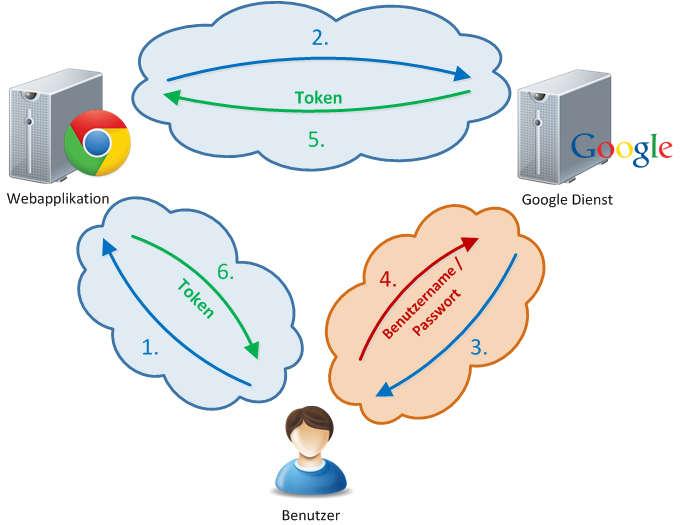
\includegraphics[width=0.7\textwidth]{images/oauth/oauth-user}
	\caption{Endbenutzer authentifiziert sich mit \gls{OAuth}}
	\label{oauth-user}
\end{figure}

Wenn der Benutzer das erste mal die gewünschte Applikation nutzen will, stellt diese fest, dass der Benutzer noch nicht authentifiziert ist. Zu diesem Zweck leitet die Applikation den Benutzer weiter zum Service Provider. Auf der Seite des Service Providers gibt der Benutzer seinen Benutzernamen und sein Passwort ein. Daraus wird ein sogenanntes \emph{Zugriffs-Token} generiert. Dieses Token wird anschliessend der Applikation und dem Benutzer mitgeteilt, fortan dient es dazu den Benutzer zu authentifizieren.

Die Applikation kann nun im festgelegten Rahmen direkt mit dem Token beim Service Provider auf die geschützten Ressourcen zugreifen.

In der Abbildung \ref{oauth-user} wird dieser Ablauf nochmals visualisiert.

\subsection{OAuth Szenarien}
Es gibt grundsätzlich verschiedene Methoden bei \gls{OAuth}, je nachdem welches Ziel eine Applikation verfolgt. Auch wenn sich der in Abschnitt \ref{oauth-authentication} beschriebene Ablauf immer ähnelt, gibt es Unterschiede im Detail.

\subsubsection{Clientseitiges OAuth}
Das clientseitige \gls{OAuth} entspricht dem im Abschnitt \ref{oauth-authentication} beschriebenen Ablauf. Ein Benutzer ist aktiv, führt die Authentifizierung durch und überlässt dann die weiteren Zugriffe der Applikation.

\subsubsection{Serverseitiges OAuth}
\label{oauth-authentication-server}
Beim serverseitigen \gls{OAuth} spielt der Endbenutzer eine untergeordnete Rolle, da er an der Authentifizierung nicht beteiligt ist. Hier geht es darum, dass sich eine Applikation gegenüber einem Service Provider authentifiziert, um auf ihre eigene Dienste zuzugreifen. Dies ist z.B. dann der Fall wenn eine Applikation als Datenbank eine \gls{Cloud}-Datenbank verwendet. Dieser Ablauf wird in der Abbildung \ref{oauth-serviceaccount} visualisiert.

\begin{figure}[!ht]
	\centering
	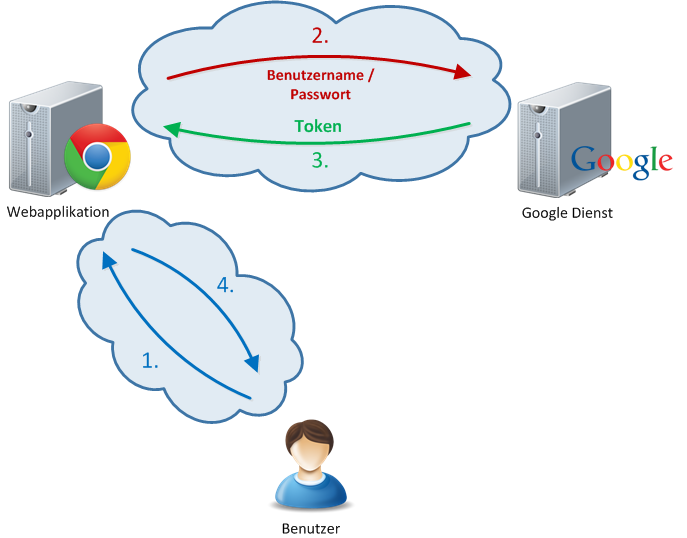
\includegraphics[width=0.7\textwidth]{images/oauth/oauth-serviceaccount}
	\caption{Applikation verwendet einen Service Account zur Authentisierung. Der Endbenutzer merkt davon nichts.}
	\label{oauth-serviceaccount}
\end{figure}

\subsection{OAuth in Google Fusion Tables}
Wir standen vor der Herausforderung die Authentifizierung für die GFT nutzbar zu machen. Für den Zugriff auf Tabellen eines Benutzers funktionierte dies ausgezeichnet, wir haben dies mit einer Beispielapplikation ausprobiert. Der Ablauf dafür ist bereits ausführlich dokumentiert\footnote{\url{https://developers.google.com/fusiontables/docs/articles/oauthfusiontables}}, so dass wenn die Konzepte klar sind mit Hilfe einer Client Library\footnote{\url{https://developers.google.com/accounts/docs/OAuth2\#libraries}} sehr einfach eine Authentisierung erstellt werden kann.

\subsubsection{FixMyStreet Use Case}
Für den Use Case FixMyStreet (siehe Kapitel \ref{fixmystreet}) waren wir jedoch vor eine neue Hürde gestellt: Wir haben GFT explizit als Applikationsdatenbank ausgelegt, so dass die Tabelle eines Benutzers alle Daten der Applikation hält. Die Applikation soll für den Endbenutzer ohne Authentifizierung benutzbar sein.

Google stellt für diesen Fall seit März 2012 sogenannte \emph{Service Accounts}\footnote{Google Developer Blog - Service Accounts have arrived: \url{http://googledevelopers.blogspot.com/2012/03/service-accounts-have-arrived.html}} zur Verfügung. Sie sind ein Beispiel für das serverseitige \gls{OAuth} (siehe Abschnitt \ref{oauth-authentication-server}).

Die Dokumentation dieses neuen Features ist leider so gut wie inexistent. Gerade auch für Google Fusion Tables fehlt ein entsprechender Service in den Client Libraries.

Die Idee bei den Service Accounts ist, dass dieser spezielle Account sich beim Service Provider anmeldet und zwar mit Hilfe eines verschlüsselten Requests. Beim erstellen des Accounts wird ein Schlüsselpaar generiert. Mit dem privaten Schlüssel können dann verschlüsselte Requests erstellt werden.

\subsubsection{OAuth in der GftLib}
Da sich für die Service Accounts die Token nur via Server erstellen lassen, haben wir einen Web Service erstellt, welcher jeweils ein gültiges Token über eine \gls{JSONP}-Schnittstelle zur Verfügung stellt. Mit dem so erworbenen Token, kann sich die JavaScript Bibliothek GftLib bei Google Fusion Tables authentifizieren. Durch die Berechtigungen auf einer Tabelle bzw. durch den Einsatz von Views können die Möglichkeiten, welches das Token bietet, eingeschränkt werden.